\chapter{Implementation}

The prototype has been implemented using an Arduino, which is connected to a circuit board with a specific sensor. 
The sesnor attached to the circuit board is called MPU 9150, and utilises a gyroscope, magnetometer, and accelorometer \citep{MPU}.

Schematic 

\begin{minipage}{\linewidth}% to keep image and caption on one page
\makebox[\linewidth]{%        to center the image
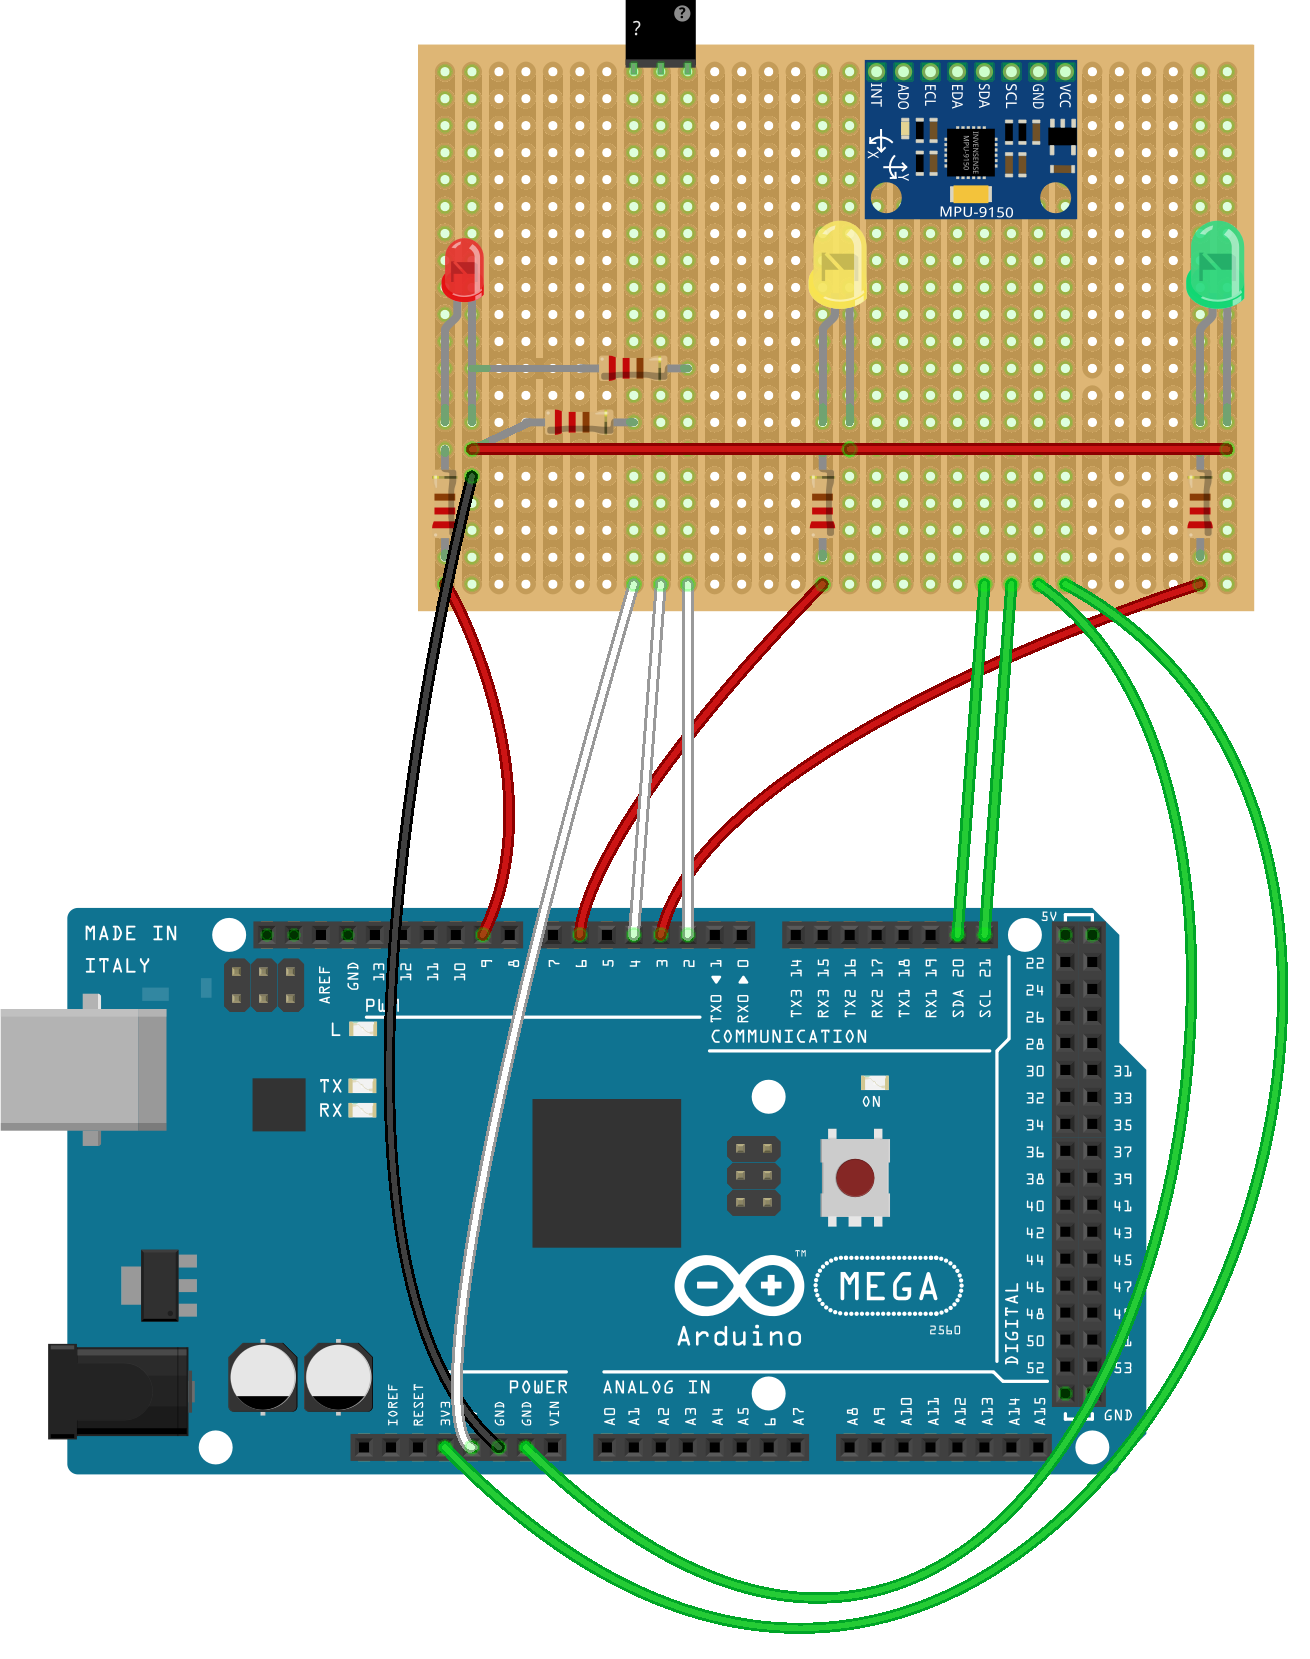
\includegraphics[keepaspectratio=true,scale=0.4]{Imu_Glove_Schematic}}
\captionof{figure}{Prototype Schematic\citep{TC}}\label{schematic}
\end{minipage}\\